\documentclass{beamer}

\mode<presentation> {
  \usetheme{Madison}
  \usefonttheme[onlymath]{serif}
}

% % % % to make navigation two lines
\usepackage{ragged2e}

\makeatletter
\setbeamertemplate{section in head/foot}{%
	\parbox[c][0.33cm][t]{\dimexpr(\textwidth-1.3cm)/\beamer@sectionmax\relax}{%
		\RaggedRight\fontsize{4}{4}\selectfont\insertsectionhead}}
\setbeamertemplate{footline}[frame number]
\makeatother
% % % %
\usepackage{booktabs, calc, rotating}
\usepackage{scalefnt}
\usepackage[english]{babel}
\usepackage[latin1]{inputenc}
\usepackage{times}
\usepackage{alltt}

  \setbeamertemplate{navigation symbols}{}
  \setbeamertemplate{blocks}[rounded][shadow=true]

%%%%%%%%%%%%%%%%%%%%%%%%%%%%%%%%%%%%%%%%%%%%%%%%%%%%%%%%%%%%%%%%%%%%%%%%%%%%%%%%%%%%
%  CHANGE THE TITLE AND INPUT FILE ACCORDING TO THE CHAPTER THAT YOU WISH TO COMPILE
%%%%%%%%%%%%%%%%%%%%%%%%%%%%%%%%%%%%%%%%%%%%%%%%%%%%%%%%%%%%%%%%%%%%%%%%%%%%%%%%%%%%

\title[Model Selection]{Model Selection and Inference}

\date[Fall 2017]{Fall 2017}
%Personal definitions
\def\bsb{\boldsymbol \beta}
\def\bsa{\boldsymbol \alpha}
\def\bsm{\boldsymbol \mu}
\def\bsS{\boldsymbol \Sigma}
\def\bsx{\boldsymbol \xi}

\begin{document}

\frame{\titlepage}

\begin{frame}
  \frametitle{Outline}\scalefont{0.8}
     \tableofcontents[part=1]\scalefont{1.25}
\end{frame}

\part<presentation>{Main Talk}
\section{Nonparametric Estimation Tools}\label{S:NonParTools}

\subsection{Moments}
\begin{frame}%[shrink=2]
\frametitle{Nonparametric Estimation} \textbf{Basic Assumption}
\vspace{4mm}

\begin{itemize}
\item $X_1, \ldots, X_n$ is a random sample (with replacement) from
F(.) \vspace{4mm}

\item Sometimes we say that $X_1, \ldots, X_n$ are identically and independently distributed
($iid$) \vspace{4mm}
\end{itemize}

We will not assume a parametric form for the distribution function F() and so proceed with a \textit{nonparametric} analysis
\vspace{4mm}

Nonparametric estimation is also referred to as ``empirical estimation''
\end{frame}

\begin{frame}%[shrink=2]
\frametitle{Moment Estimators}
\begin{itemize}
\item The $k$th raw moment is $\mathrm{E~} X^k = \mu^{\prime}_k$ \vspace{4mm}

\item It is nonparametrically estimated by the corresponding statistic
$$ \frac{1}{n} \sum_{i=1}^n X_i^k $$ \vspace{4mm}

\item The $k$th central moment is $\mathrm{E~} (X-\mu)^k = \mu_k$ \vspace{4mm}

\item It is nonparametrically estimated by the corresponding statistic
$$ \frac{1}{n} \sum_{i=1}^n \left(X_i-\bar{X}\right)^k $$
\end{itemize}
\end{frame}

\begin{frame}%[shrink=2]
\frametitle{Empirical Distribution Function}
\begin{itemize}\scalefont{1}
\item Define the \textbf{empirical distribution function} to be
\begin{eqnarray*}
F_n(x) &=& \frac{\text{number of observations less than or equal to }x}{n} \\
&=& \frac{1}{n} \sum_{i=1}^n I\left(X_i \le x\right).
\end{eqnarray*}
Here, the notation $I(\cdot)$ is the indicator function, it returns 1 if the event $(\cdot)$ is true and 0 otherwise.
\item\textbf{Example -- Toy}. Consider $n=10$ observations:

\begin{table}[H]\begin{center}\scalefont{0.8}
    \begin{tabular}{l|cccccccccc}
    \hline
$i$ &1&2&3&4&5&6&7&8&9&10 \\
$X_i$& 10 &15 &15 &15 &20 &23 &23 &23 &23 &30\\
    \hline
    \end{tabular}\end{center} \end{table}
\item The nonparametric estimate of the mean (\textbf{sample mean}) is $\bar{x} = 19.7$, and the nonparametric estimate of the second central moment (\textbf{sample variance}) is
31.01
\end{itemize}

\end{frame}

\begin{frame}[shrink=2]
\frametitle{Empirical Distribution Function II}
\begin{figure}[htp]
\begin{center}
    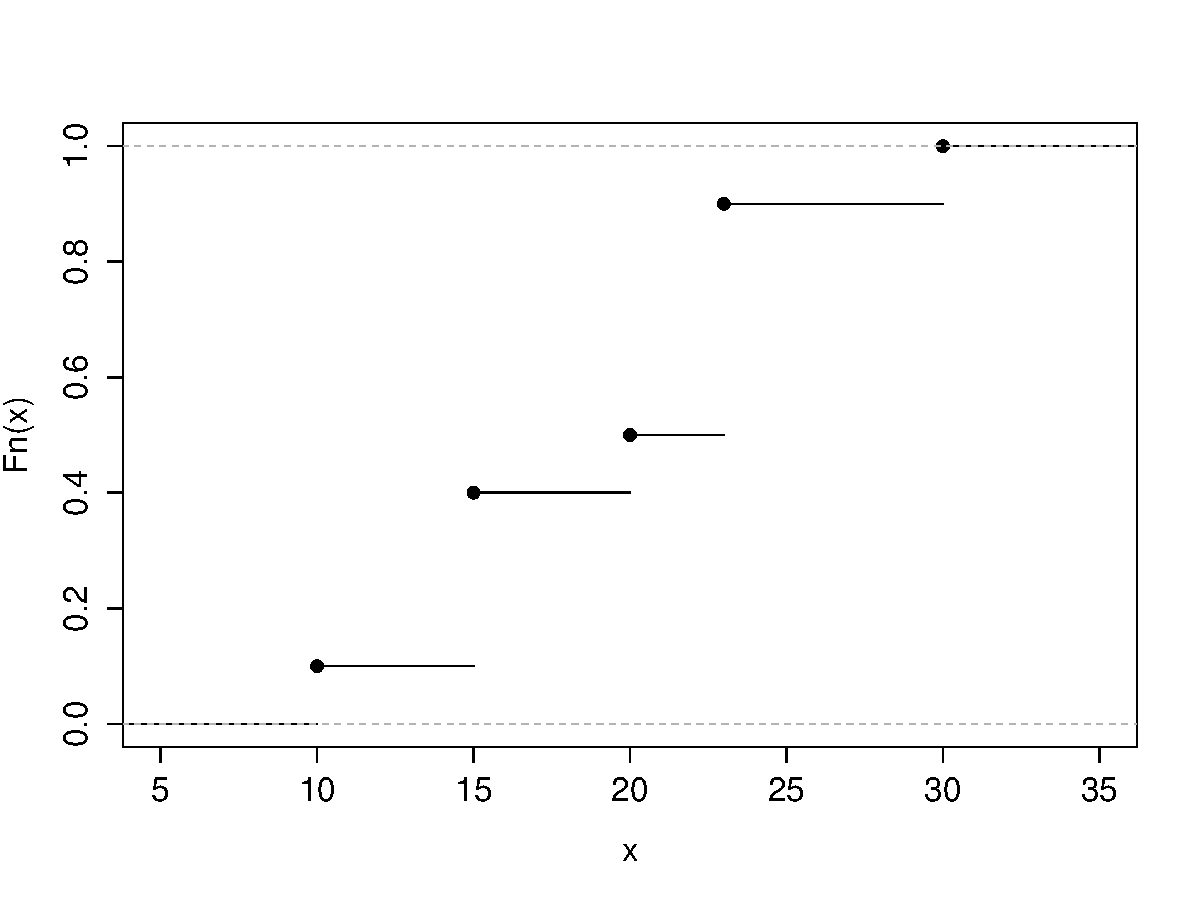
\includegraphics[scale = 0.4, bb = 600 520 100 100]{Figures/EDFExample.pdf}
     \caption{\label{F:EDFToy}Empirical Distribution Function of a Toy Example}
\end{center}
\end{figure}
\end{frame}

\subsection{Quantiles}

\begin{frame}[shrink=2]
\frametitle{Percentiles I}
\begin{itemize}
\item Special Cases \vspace{4mm}

\begin{itemize}
\item The \textit{median} is that number so that half of a data set is below (or above)
it \vspace{4mm}

\item The first \textit{quartile} is that number so that 25\% of the data is below
it \vspace{4mm}

\item A $100q$ \textit{percentile} is that number so that $100 \times q$ percent of the data is below
it \vspace{4mm}

\end{itemize}
\item In general, for a given $0<q<1$, define the \textbf{$100q$th percentile (or quantile)}, $q_F$, to be any number that satisfies
\begin{eqnarray*}
F(q_F-) \le q \le F(q_F)
\end{eqnarray*} \vspace{4mm}

Here, the notation $F(x-)$ means to evaluate the function $F(\cdot)$
as a left-hand limit \vspace{4mm}

\item If $F(\cdot)$ is continuous at $q_F$, then $F(q_F-) = F(q_F)$
\end{itemize}

\end{frame}

\begin{frame}[shrink=2]
\frametitle{Percentiles II}
\begin{itemize} \vspace{5mm}

\item If F is smooth or there is a jump at $q$, the definition of the percentile $q_F$ is
unique \vspace{4mm}

\item If F is flat at $q$, then there a many definitions of $q_F$ \vspace{20mm}

\end{itemize}
\begin{figure}[h]
\begin{center}
    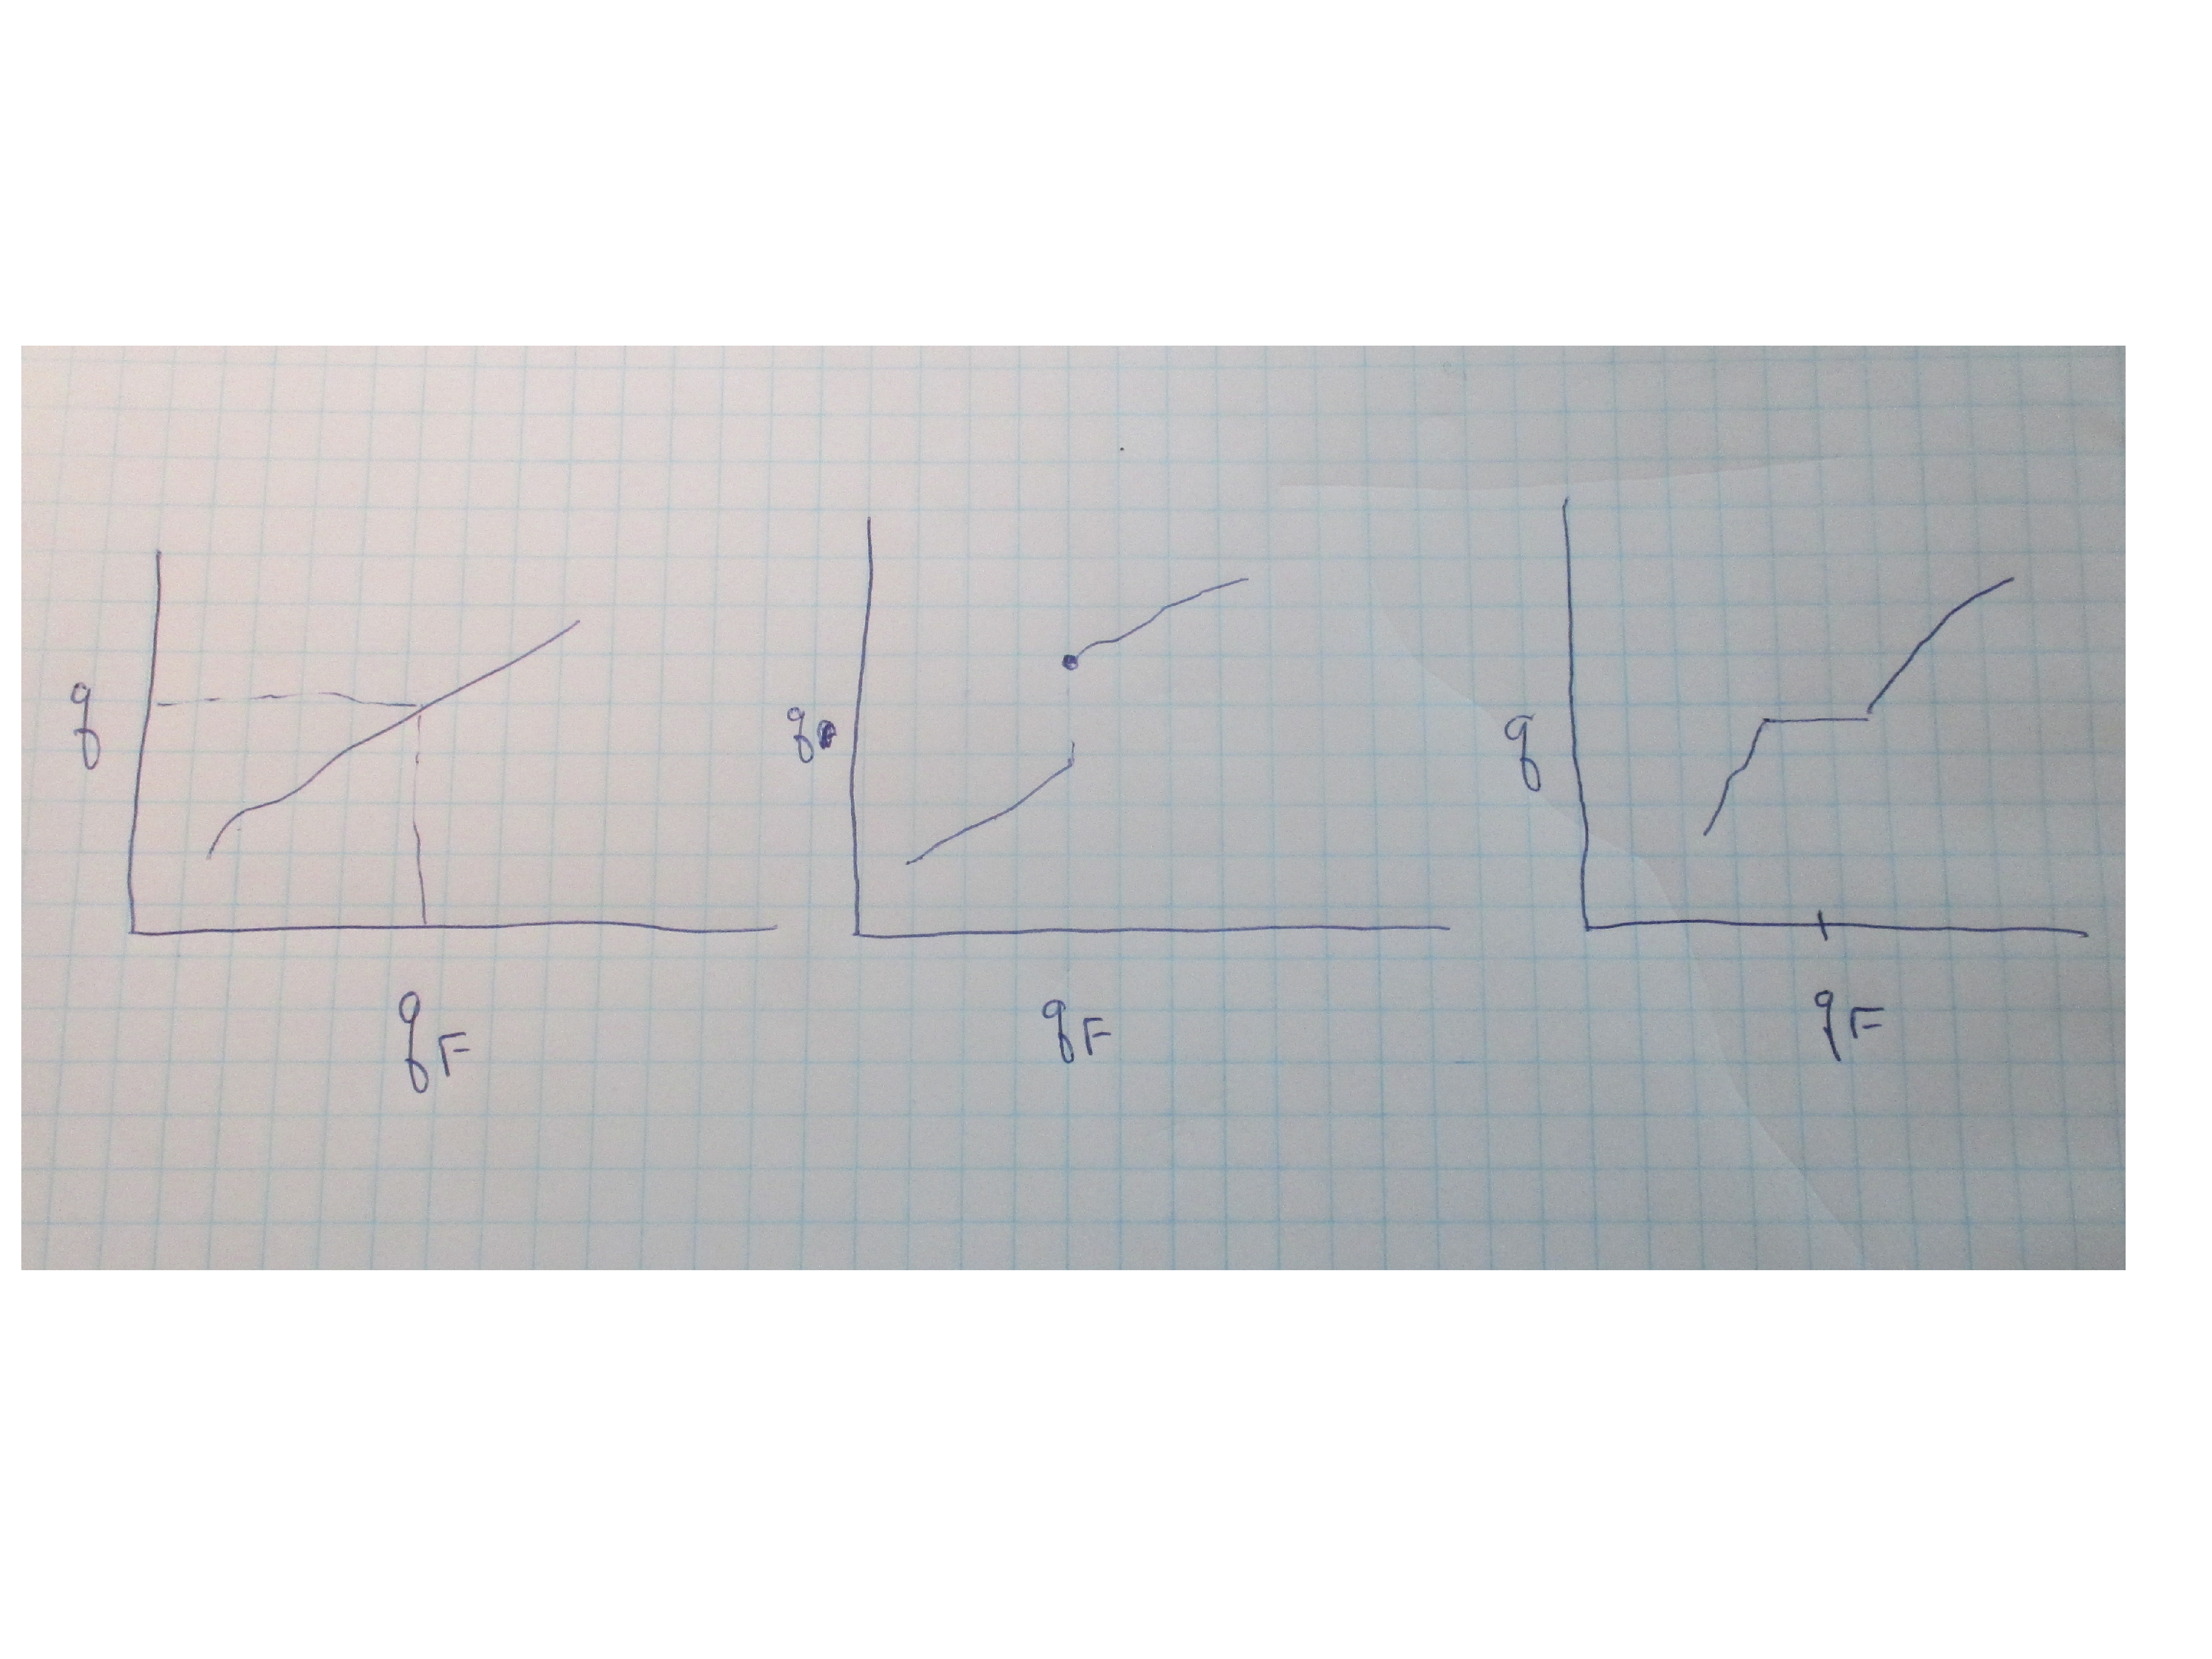
\includegraphics[scale = 0.15, bb = 800 220 800 400]{Figures/ThreeQuantileCases.pdf}
\end{center}
\end{figure}
\end{frame}

\begin{frame}[shrink=2]
\frametitle{Smoothed Empirical Percentiles I} \textbf{Example --
Toy}. Consider $n=10$ observations:

\begin{table}[H]\begin{center}\scalefont{0.8}
    \begin{tabular}{l|cccccccccc}
    \hline
$i$ &1&2&3&4&5&6&7&8&9&10 \\
$X_i$& 10 &15 &15 &15 &20 &23 &23 &23 &23 &30\\
    \hline
    \end{tabular}\end{center} \end{table} \vspace{4mm}

\begin{itemize}
\item The median might be defined to be any number between 20 and 23
\vspace{4mm}
\begin{itemize}
\item Many software packages use the average 21.5 \end{itemize} \vspace{4mm}
\item KPW defines the \textit{smoothed empirical percentile} to be
$$ \hat{\pi}_q = (1-h) X_{(j)} + h X_{(j+1)}$$ \vspace{2mm}
where $j=[(n+1)q]$ and, $h=(n+1)q-j$, and $X_{(1)}, \ldots, X_{(n)}$
are the ordered values (the \textit{order statistics}) corresponding
to $X_1, \ldots, X_n$ \end{itemize}
\end{frame}

\begin{frame}[shrink=2]
\frametitle{Smoothed Empirical Percentiles II} \textbf{Example --
Toy}. Take $n=10$ and $q=0.5$. Then, \vspace{4mm}

\begin{itemize}

\item $j=[(11)0.5]=[5.5]=5$ and, $h=(11)(0.5)-5=0.5$ \vspace{4mm}

\item
$$ \hat{\pi}_{0.5} = (1-0.5) X_{(5)} + (0.5) X_{(6)} = 0.5 (20) + (0.5)(23) =
21.5$$ \vspace{4mm}
\end{itemize}

Take $n=10$ and $q=0.2$. Then, \vspace{4mm}
\begin{itemize}
\item $j=[(11)0.2]=[2.2]=2$ and  $h=(11)(0.2)-2=0.2$ \vspace{4mm}

\item $$ \hat{\pi}_{0.2} = (1-0.2) X_{(2)} + (0.2) X_{(3)} = 0.2 (15)
+ (0.8)(15) = 15$$
\end{itemize}
\end{frame}


\subsection{Density Estimators}

\begin{frame}[shrink=2]
\frametitle{Density Estimators}
\begin{itemize}
\item When the random variable is discrete, estimate the probability mass function $f(x) = \Pr(X=x)$ is using
$$ f_n(x) = \frac{1}{n} \sum_{i=1}^n I(X_i = x).$$
\item Observations may be ``grouped'' in the sense that they fall into intervals of the form $[c_{j-1}, c_j)$, for $j=1, \ldots, k$. The constants $\{c_0 < c_1 < \cdots < c_k\}$ form some partition of the domain of F(.).
 \item    Then, use
$$ f_n(x) = \frac{n_j}{n \times (c_j - c_{j-1})}  \ \ \ \ \ \ c_{j-1} \le x < c_j,$$
where $n_j$ is the number of observations ($X_i$) that fall into the interval $[c_{j-1}, c_j)$.
\item Another way to write this is
$$  f_n(x) = \frac{1}{n(c_j-c_{j-1})} \sum_{i=1}^n I(c_{j-1} < X_i \le c_j).$$
\end{itemize}
\end{frame}

\begin{frame}[shrink=2]
\frametitle{Uniform Kernel Density Estimator}
\begin{itemize}
\item Let $b>0$, known as a ``bandwidth,''
\begin{eqnarray*}
 f_n(x) = \frac{1}{2nb} \sum_{i=1}^n I(x-b < X_i \le x + b).
\end{eqnarray*}
\item The estimator is the average over $n$ $iid$ realizations of a random variable with mean
\begin{eqnarray*}
\mathrm{E~ } \frac{1}{2b} I(x-b < X \le x + b) &=& \frac{1}{2b}\left(F(x+b)-F(x-b)\right) \\
&=& \frac{1}{2b} \left( \left\{ F(x) + b F^{\prime}(x) + b^2 C_1\right\} \right.\\
&& \ \ \ -
\left. \left\{ F(x) - b F^{\prime}(x) + b^2 C_2\right\} \right) \\
&=& F^{\prime}(x) + b \frac{C_1-C_2}{2} \rightarrow  F^{\prime}(x) = f(x),
\end{eqnarray*}
as $b\rightarrow  0$. That is, $f_n(x)$ is an asymptotically unbiased estimator of $f(x)$.
\end{itemize}
\end{frame}

\begin{frame}
\frametitle{Kernel Density Estimator}
\begin{itemize}
\item More generally, define the \textbf{kernel density estimator}
\begin{eqnarray*}
 f_n(x) = \frac{1}{nb} \sum_{i=1}^n k\left(\frac{x-X_i}{b}\right)
\end{eqnarray*}
where $k$ is a probability density function centered about 0


\item Special Cases
\begin{itemize}
\item uniform kernel: $k(x) = \frac{1}{2}I(|x| \le 1)$,

\item triangular kernel: $k(x) = (1-|x|)\times I(|x| \le 1)$,

\item Epanechnikov kernel: $k(x) = \frac{3}{4}(1-x^2) \times I(|x| \le 1)$, 

\item Gaussian kernel: $k(x) = \phi(x)$, where $\phi(\cdot)$ is the standard normal density function
\end{itemize}\end{itemize}
\end{frame}


\begin{frame}
\frametitle{Kernel Density Estimator of a Distribution Function}
\begin{itemize}
\item The kernel density estimator of a \textbf{distribution function} is
\begin{eqnarray*}
 \hat{F}_n(x) = \frac{1}{n} \sum_{i=1}^n K\left(\frac{x-X_i}{b}\right).
\end{eqnarray*}
where $K$ is a probability distribution function associated with the kernel density $k$.
\item To illustrate, for the uniform kernel, we have $k(y) = \frac{1}{2}I(-1 < y \le 1)$ so
\begin{eqnarray*}
K(y) =
\begin{cases}
0 &            y<-1\\
\frac{y+1}{2}& -1 \le y < 1 \\
1 & y \ge 1 \\
\end{cases}
\end{eqnarray*}
\end{itemize}
\end{frame}

\section{Nonparametric Estimation Tools For Model Selection}

\subsection{Graphical Comparisons}

\begin{frame}[shrink=2]
\frametitle{Comparing Distribution and Density Functions}
\begin{itemize}
\item The left-hand panel compares distribution functions, with the dots corresponding to the empirical distribution, the thick blue curve corresponding to the fitted gamma and the light purple curve corresponding to the fitted Pareto.
\item The right hand panel compares these three distributions summarized using probability density functions.
\end{itemize}
%\vspace{-.2in}
\begin{figure}[htp]
\begin{center}
    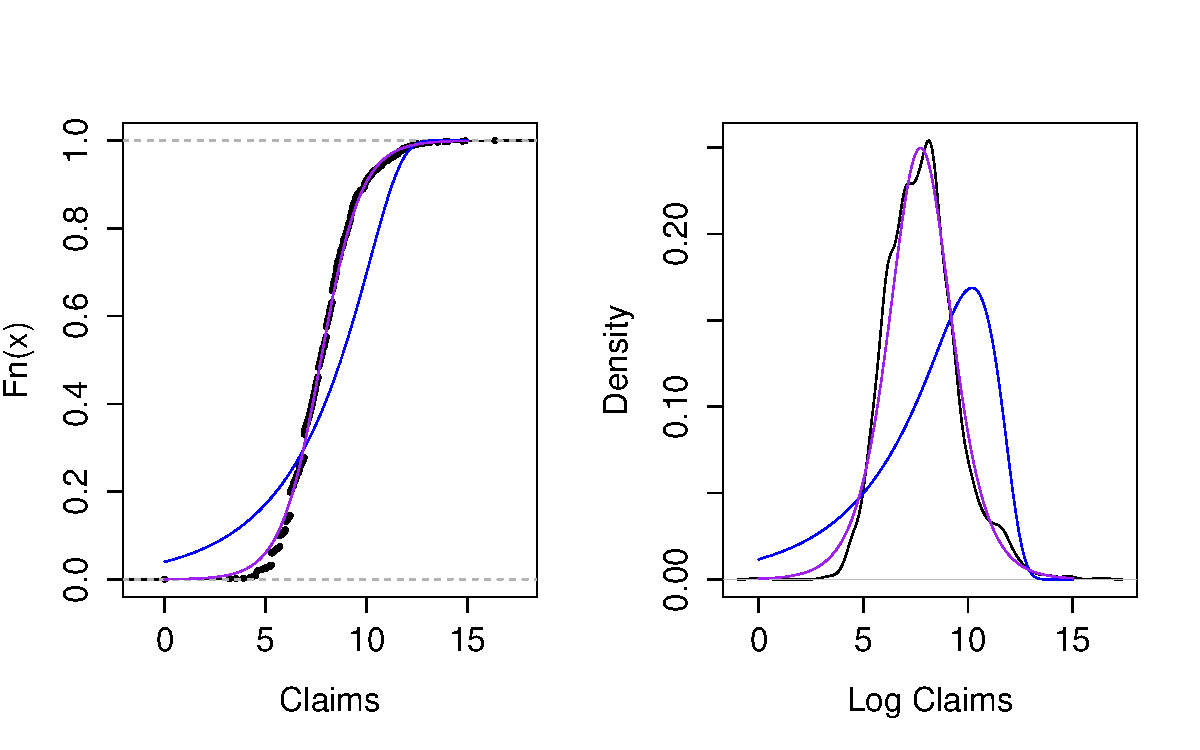
\includegraphics[width=.6\textwidth]{Figures/ComparisonCDFPDF.pdf}
     \caption{\label{F:ComparisonCDFPDF}Nonparametric Versus Fitted Parametric Distribution and Density Functions.}
\end{center}
\end{figure}
\end{frame}


\begin{frame}[shrink=2]
\frametitle{\textit{PP} Plot}
\begin{itemize}
\item  The horizontal axes gives the empirical distribution function at each observation.
\item In the left-hand panel, the corresponding distribution function for the gamma is shown in the vertical axis. \item  The right-hand panel shows the fitted Pareto distribution. Lines of $y=x$ are superimposed.
\end{itemize}

\vspace{-.1in}
\begin{figure}[htp]
\begin{center}
    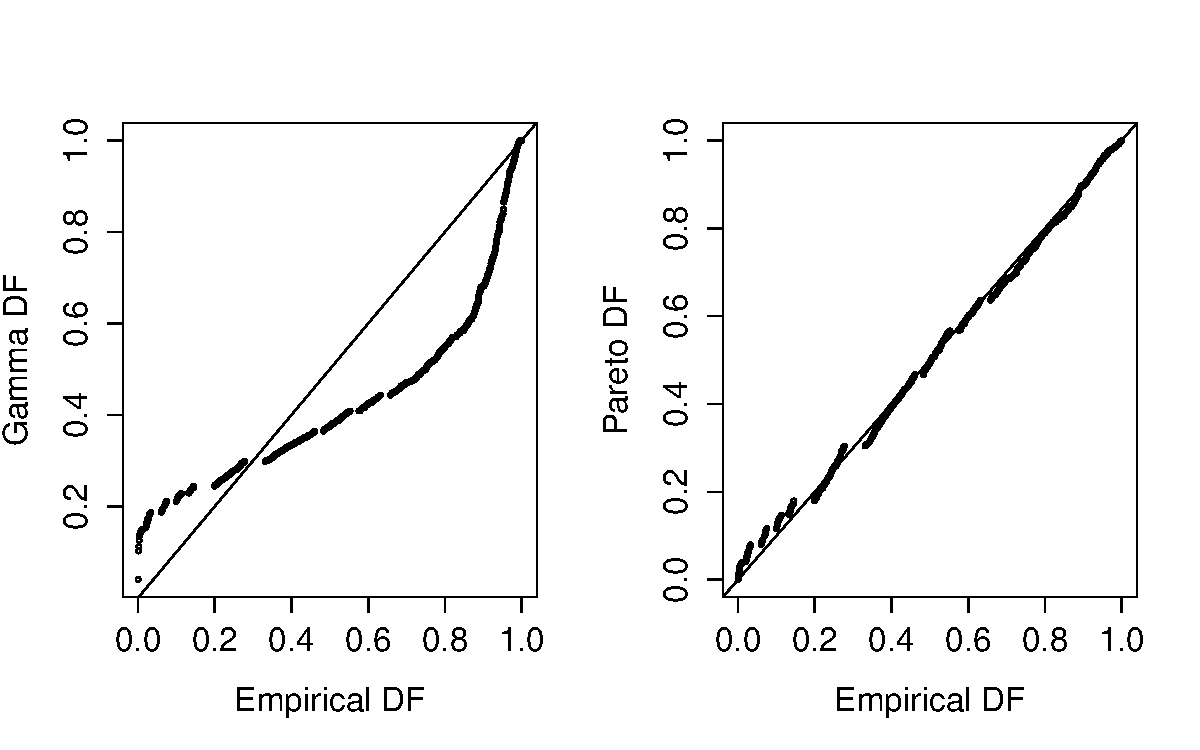
\includegraphics[width=.6\textwidth]{Figures/PPPlot.pdf}
     \caption{\label{F:PPPlot}Probability-Probability ($pp$) Plots.}
\end{center}
\end{figure}
\textbf{KPW} also recommends plotting the difference $D(x) = F_n(x) - F^*(x)$ versus $x$. Here, $F^*(x)$ is the fitted model distribution function.
\end{frame}

\begin{frame}%[shrink=2]
\frametitle{\textit{QQ} Plot}
\begin{itemize}\scalefont{0.8}
\item The horizontal axes gives the empirical quantiles at each observation.
\item The right-hand panels they are graphed on a logarithmic basis.
\item The vertical axis gives the quantiles from the fitted distributions; Gamma quantiles are in the upper panels, Pareto quantiles are in the lower panels.
\item The lower-right hand panel suggests that the Pareto distribution does a good job with large observations but provides a poorer fit for small observations.
\end{itemize}
\vspace{-.1in}
\begin{figure}[htp]
\begin{center}
    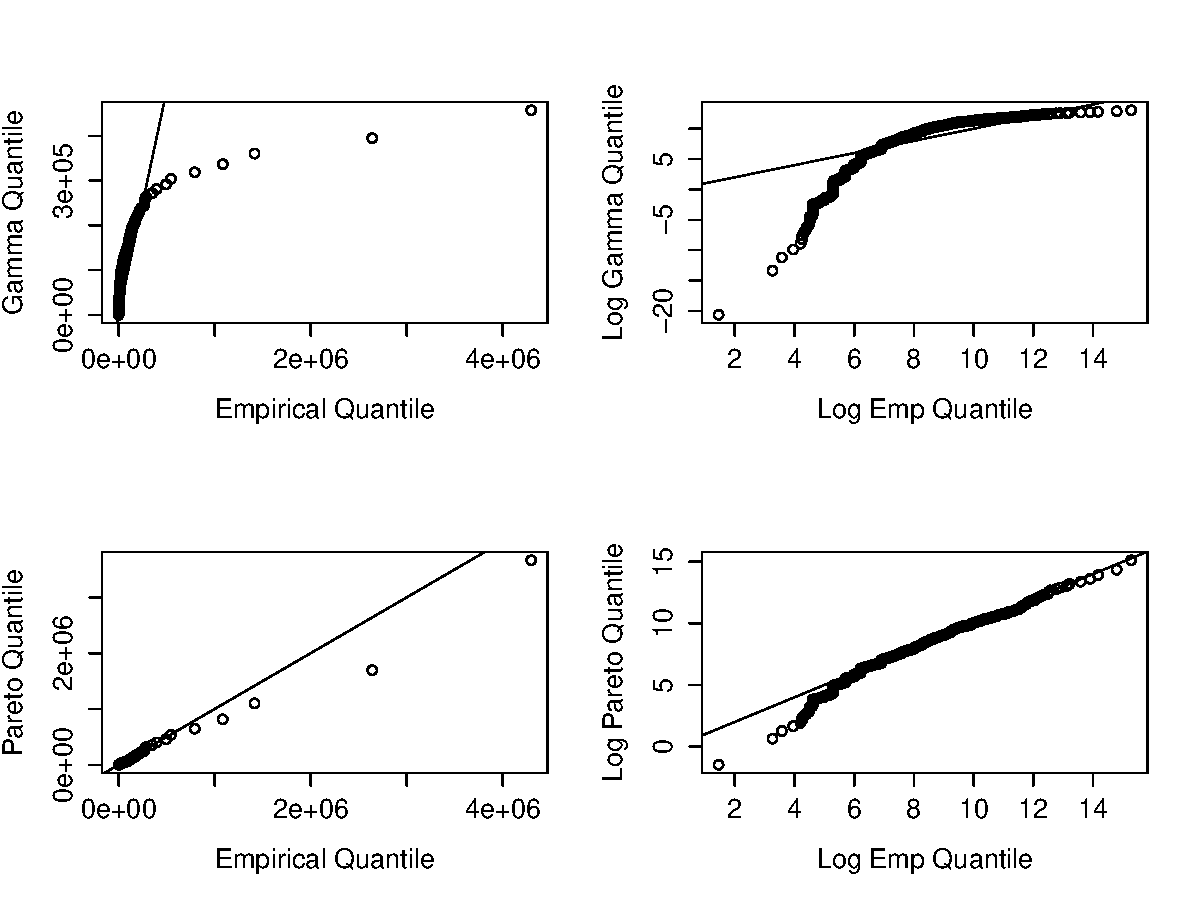
\includegraphics[width=.6\textwidth]{Figures/QQPlot.pdf}
     \caption{\label{F:QQPlot}Quantile-Quantile ($qq$) Plots.}
\end{center}
\end{figure}
\end{frame}

\subsection{Statistical Comparisons}

\begin{frame}%[shrink=2]
\frametitle{Three Goodness of Fit Statistics}
\begin{table}[H]\scalefont{0.8}
 \centering
    \begin{tabular}{l|cc}
    \hline
Statistic & Definition & Computational Expression \\ \hline
 Kolmogorov& $sup_x |F_n(x) - F(x) | $ & $max(D^+ - D^-)$  \ \text{where } \\
 ~~~-Smirnov &&$D^+ = max_{i=1, \ldots, n} \left(\frac{i}{n} - F_i\right)$ \\
  &&$D^- = max_{i=1, \ldots, n} \left(F_i - \frac{i-1}{n} \right)$ \\\hline
Cramer& $ n \int (F_n(x) - F(x))^2 dx$ & $\frac{1}{12n} + \sum_{i=1}^n \left(F_i - (2i-1)/n\right)^2 $ \\
~~~-von Mises \\ \hline
Anderson& $ n \int \frac{(F_n(x) - F(x))^2}{F(x)(1-F(x))} dx$ & \multicolumn{1}{l}{$-n $} \\
~~~-Darling &  & $-\frac{1}{n} \sum_{i=1}^n (2i-1) \log\left(F_i(1-F_{n+1-i})\right)^2 $ \\
    \hline
    \multicolumn{3}{l}{where $F_i$ is defined to be $F(x_i)$.}
    \end{tabular}
 \end{table}
\end{frame}

\section{Nonparametric Estimation using Modified Data}

\subsection{Grouped Data}
\begin{frame}%[shrink=2]
\frametitle{Grouped Data}
\begin{itemize}\scalefont{0.9}
\item Observations may be ``grouped'' in the sense that they fall into intervals of the form $[c_{j-1}, c_j)$, for $j=1, \ldots, k$.
\item The constants $\{c_0 < c_1 < \cdots < c_k\}$ form some partition of the domain of F(.).
\item Define the empirical distribution function at the boundaries is defined in the usual way:
$$ F_n(c_j) = \frac{\text{number of observations } \le c_j}{n} $$
\item For other values of $x$, one could use the

\textbf{Ogive:} connect values of the boundaries with a straight line.
\item For another way of smoothing, recall the kernel density estimator of the distribution function
\begin{eqnarray*}
 \hat{F}_n(x) = \frac{1}{n} \sum_{i=1}^n K\left(\frac{x-X_i}{b}\right).
\end{eqnarray*}
 \item    For densities, use
$$ f_n(x) = \frac{n_j}{n \times (c_j - c_{j-1})}  \ \ \ \ \ \ c_{j-1} \le x < c_j,$$
\end{itemize}

\end{frame}

\subsection{Censored Data}

\begin{frame}[shrink=.5]
\frametitle{Censored Data}
\begin{itemize}
\item Censoring occurs when we observe only a limited value of an observation.
\item Suppose that $X$ represents a loss due to an insured event and that $u$ is a known censoring point.
\item If observations are censored from the \textbf{right} (or from above), then we observe
$$ Y = \min(X,u).$$
\vspace{-.2in}
\begin{itemize}\scalefont{0.9}
\item In this case, $u$ may represent the upper limit of coverage for an insurer. The loss exceeds the amount $u$ but the insurer does not have in its records the amount of the actual loss.\end{itemize}
\item If observations are censored from the \textbf{left} (or from below), then we observe
$$ Y = \max(X,u).$$
\vspace{-.2in}
\begin{itemize}\scalefont{0.9}
\item Let $u$ represents the upper limit of coverage but now $Y - u$ represents the amount that a \textit{reinsurer} is responsible for. If the loss $X < u$, then $Y=0$, no loss for the reinsurer. If the loss $X  \ge u$, then $Y= X-u$ represents the reinsurer's retained claims.  \end{itemize}
\end{itemize}
\end{frame}

\begin{frame}[shrink=.22]
\frametitle{Kaplan-Meier Product Limit Estimator}
\begin{itemize}
\item  Let $t_{1} <\cdots< t_{c}$ be distinct points at which an event of interest occurs, or non-censored losses, and let $s_j$ be the number of events at time point $t_{j}$ .
\item  Further, the corresponding ``risk set'' is the number of observations that are active at an instant just prior to $t_{j}$ . Using notation, the risk set is $R_{j}=\sum_{i=1}^{n}I(x_{i}\geq t_{j})$.
\item  With this notation, the \textbf{product-limit estimator} of the distribution function is
$$
\hat{F}(x)=
\left\lbrace
\begin{array}{llll}
0 &
x < t_{1} \\
1-\prod_{j:t_{j} \leq x}\left( 1-\frac{s_j}{R_{j}}\right)  &
x \geq t_{1} .\\
\end{array}
\right .
$$
\item Greenwood (1926) derived the formula for the estimated variance
$$ \widehat{Var}(\hat{F}(x)) =
(1-\hat{F}(x))^{2}
\sum _{j:t_{j} \leq x} \dfrac{s_j}{R_{j}(R_{j}-s_j)}.$$
\end{itemize}
\end{frame}

\subsection{Truncated Data}

\begin{frame}[shrink=.22]
\frametitle{Truncated Data}
\begin{itemize}
\item An outcome is potentially \textbf{truncated} when the availability of an observation depends on the outcome.
\item In insurance, it is common for observations to be truncated from the \textbf{left} (or below) at $d$ when the amount observed is
\begin{equation*}
Y = \begin{cases}
\text{we do not observe X}  &  X < d\\
X-d                         &   X \ge d.
\end{cases}
\end{equation*}
\vspace{-.2in}
\begin{itemize}\scalefont{0.9}\item In this case, $d$ may represent the deductible associated with an insurance coverage. If the insured loss is less than the deductible, then the insurer does not observe the loss. If the loss exceeds the deductible, then the excess $X-d$ is the claim that the insurer covers.
\end{itemize}
\item Observations may also truncated from the \textbf{right} (or above) at $d$ when the amount observed is
\begin{equation*}
Y = \begin{cases}
X   &   X < d  \\
\text{we do not observe X}  &  X \ge d\\
\end{cases}
\end{equation*}
\vspace{-.2in}
\begin{itemize}\scalefont{0.9}\item Classic examples of truncation from the right include $X$ as a measure of distance of a star. When the distance exceeds a certain level $d$, the star is no longer observable.\end{itemize}
\end{itemize}
\end{frame}

\begin{frame}%[shrink=.22]
\frametitle{Right-Censored, Left-Truncated Empirical Distribution Functions}
\begin{itemize}\scalefont{0.9}
\item Procedure from \textbf{KPW}. Notation:
\begin{itemize} \scalefont{0.8}
\item For each observation $i$, let $d_i$ be the lower truncation limit (0 if no truncation)
\item Let $u_i$ be the upper censoring limit (=$\infty$ if no censoring)
\item The recorded value is $x_i$ in the case of no censoring, $u_i$ if there is censoring.
\item For notation, let $t_1 < \cdots < t_k$ be $k$ unique observations of $x_i$ that are uncensored.
\item Define $s_j$ to be the number of $x_i$'s at $t_j$.
\item  Define the risk set
$$R_j = \sum_{i=1}^n I(x_i \geq t_{j}) + \sum_{i=1}^n I(u_i \geq t_{j}) - \sum_{i=1}^n I(d_i \geq t_{j})$$
\end{itemize}
\item  The product-limit estimator of the distribution function is
\[
\hat{F}(x)=
\left\lbrace
\begin{array}{llll}
0 &
x < t_{1} \\
1- \prod_{j:t_{j} \leq x}\left( 1-\frac{s_j}{R_{j}}\right)  &
x \geq t_{1}\\
\end{array}
\right .
\]
\item  The Nelson-\"{A}alen estimator of the distribution function is
$$\hat{F}(x)=
\left\lbrace
\begin{array}{llll}
0 &
x < t_{1} \\
1- \exp \left(-\sum_{j:t_{j} \leq x}\frac{s_j}{R_j} \right) &
x \geq t_{1}\\
\end{array}
\right.$$
\end{itemize}

\end{frame}

\section{Topics in Parametric Estimation}

\subsection{Starting Values}

\begin{frame}%[shrink=2]
\frametitle{Starting Values}
\begin{itemize}
\item Maximum likelihood is a desirable estimation technique because
\begin{itemize}
\item It employs data efficiently (enjoys certain optimality properties)
\item It can be used in a variety of data sampling schemes (e.g.,\textit{iid}, grouped, censored, regression, and so forth)
\end{itemize}
\item However, maximum likelihood is a recursive estimation procedure that requires starting values to begin the recursion
\item Two alternative estimation techniques are:
\begin{itemize}
\item Method of moments
\item Percentile matching
\end{itemize}
\item These are non-recursive techniques. Easy to implement and explain. Although less efficient than maximum likelihood, they can be employed to provide starting values for maximum likelihood.
\end{itemize}
\end{frame}

\begin{frame}[shrink=2]
\frametitle{Method of Moments}
\begin{itemize}
\item Idea: Approximate the moments using a parametric distribution to the empirical (nonparametric)
moments \vspace{2mm}

\item Assume we have a random sample $X_1$, ..., $X_n$, with all observations from the
same (assumed) parametric distribution \vspace{2mm}

\item The parametric distribution has cdf $F(x;\mathbf{\theta})$, where $\mathbf{\theta}$ = ($\theta_1$, ..., $\theta_p$) is
a vector of $p$ parameters to be estimated \vspace{2mm}

\item A \textbf{method of moments} estimate of $\mathbf{\theta}$ is any solution of the $p$ equations: \vspace{2mm}

\hspace{1in} $E[X^k ]$ = $\frac{1}{n}\sum^n_{i =
1}X^k_i$ for $k$ = 1, 2, ..., $p$ \vspace{2mm}

\item In theory, any $p$ moments could be used (for example,
negative moments to estimate the parameters of an inverse
distribution)
\end{itemize}
\end{frame}

\begin{frame}%[shrink=2]
\frametitle{Method of Moments - Example}
\begin{itemize}\scalefont{0.9}
\item \textbf{Example - Property Fund.} For the 2010 property fund, there are $n=1,377$ individual claims (in thousands of dollars) with
\begin{eqnarray*}
m_1 = \frac{1}{n} \sum_{i=1}^n X_i = 26.62259 \ \ \ \
\text{and} \ \ \ \
 m_2 = \frac{1}{n} \sum_{i=1}^n X_i^2 = 136154.6 .
\end{eqnarray*}
\item Gamma Distribution
\begin{itemize}\scalefont{0.8}
\item From theory, $\mu_1 = \alpha \theta$ and $\mu_2^{\prime} = \alpha(\alpha+1) \theta^2$.
\item Equating the two yields the method of moments estimators, easy algebra shows that
\begin{eqnarray*}
\alpha = \frac{\mu_1^2}{\mu_2^{\prime}-2\mu_1^2}  \ \ \ \text{and} \ \ \  \theta = \frac{\mu_2^{\prime}-\mu_1^2}{\mu_1}.
\end{eqnarray*}
\item The method of moment estimators are
\begin{eqnarray*}
\hat{\alpha} &=& \frac{26.62259^2}{136154.6-26.62259^2} = 0.005232809\\
%\text{and} \\
\hat{\theta} &=& \frac{136154.6-26.62259^2}{26.62259} = 5,087.629.
\end{eqnarray*}
\item In contrast, the maximum likelihood values turn out to be $\hat{\alpha}_{MLE} =  0.2905959$ and $\hat{\theta}_{MLE} = 91.61378$
\item Big discrepancies between the two estimation procedures, suggesting that the gamma model fits poorly.
\end{itemize}\end{itemize}
\end{frame}


\begin{frame}%[shrink=2]
\frametitle{Method of Moments - Example II}
\begin{itemize}\scalefont{0.85}
\item \textbf{Example - Property Fund.} Recall the nonparametric estimates
\begin{eqnarray*}
m_1 = \frac{1}{n} \sum_{i=1}^n X_i = 26.62259 \ \ \ \
\text{and} \ \ \ \
 m_2 = \frac{1}{n} \sum_{i=1}^n X_i^2 = 136154.6 .
\end{eqnarray*}
\item Pareto Distribution
\begin{itemize}\scalefont{0.85}
\item From theory, $\mu_1 = \theta/(\alpha -1)$ and $\mu_2^{\prime} = 2\theta^2/((\alpha-1)(\alpha-2) )$.
\item Easy algebra shows
\begin{eqnarray*}
\alpha = 1+ \frac{\mu_2^{\prime}}{\mu_2^{\prime}-2\mu_1^2} \ \ \ \
\text{and} \ \ \ \ \
 \theta = (\alpha-1)\mu_1.
\end{eqnarray*}
\item The method of moment estimators are
\begin{eqnarray*}
\hat{\alpha} &=& 1+ \frac{136154.6}{136154.6-2*26,62259^2} = 2.01052\\
%\text{and} \\
\hat{\theta} &=& (2.01052-1) \cdot 26.62259 = 26.9027
\end{eqnarray*}
\item The maximum likelihood values turn out to be $\hat{\alpha}_{MLE} =  0.9990936$ and $\hat{\theta}_{MLE} = 2.2821147$.
\item Interesting that $\hat{\alpha}_{MLE}<1$; for the Pareto distribution; recall that $\alpha <1$ means that the mean is infinite.
\item Indicates that the property claims data set is a long tail distribution.
\end{itemize}\end{itemize}
\end{frame}

\begin{frame}[shrink=2]
\frametitle{Percentile Matching}
\begin{itemize}
\item Under percentile matching, one approximates the parametric distribution using the empirical (nonparametric) percentiles \vspace{2mm}

\item Assume we have a random sample $X_1$, ..., $X_n$, with all observations from the
same (assumed) parametric distribution \vspace{2mm}

\item The parametric distribution has cdf $F(x;\mathbf{\theta})$, where $\mathbf{\theta}$ = ($\theta_1$, ..., $\theta_p$) is
a vector of $p$ parameters to be estimated \vspace{2mm}

\item Let $g_k$ denote an arbitrarily chosen value between 0 and 1 (0\% and 100\%), for $k$ =
1, 2, ..., $p$ \vspace{2mm}

\item Let $\hat{\pi}_{g_k}$ denote an empirical estimate of the percentile that corresponds to
$g_k$ \vspace{2mm}

\item A \textbf{percentile matching} estimate of $\mathbf{\theta}$ is any
solution of the $p$ equations: \vspace{2mm}

\hspace{1in} $F[\hat{\pi}_{g_k};\mathbf{\theta}]$ = $g_k$ for $k$ =
1, 2, ..., $p$ \vspace{2mm}
\end{itemize}
\end{frame}

\begin{frame}%[shrink=2]
\frametitle{Percentile Matching - Example}
\begin{itemize}\scalefont{0.85}
\item \textbf{Example - Property Fund.}
\item The 25th percentile (the first quartile) turns out to be 0.78853 and the 95th percentile is 50.98293 (both in thousands of dollars).
\item Pareto Distribution
\begin{itemize}\scalefont{0.8}
\item The Pareto distribution is particularly intuitively pleasing because of the closed-form solution for the quantiles.
\item The distribution function is $F(x) = 1 - \left(\theta/(x+\theta )\right)^{\alpha}$.
\item Easy algebra shows that we can express the quantile as
$$F^{-1}(q) = \theta \left( (1-q)^{-1/\alpha} -1 \right) $$
for a fraction $q$, $0<q<1$.
\item With two equations
$$ 0.78853 = \theta \left( (1-.25)^{-1/\alpha} -1 \right) \ \ \ \ \text{and} \ \ \ \ 50.98293 = \theta \left( (1-.95)^{-1/\alpha} -1\right)$$
and two unknowns, the solution is $
\hat{\alpha} = 0.9412076 \ \ \ \ \ \text{and} \ \ \ \
\hat{\theta} = 2.205617 .$
\item A numerical routine was required for these solutions - no analytic solution available.
\item Recall that the maximum likelihood values are $\hat{\alpha}_{MLE} =  0.9990936$ and $\hat{\theta}_{MLE} = 2.2821147$.
\item The percentile matching provides a better approximation for the Pareto distribution than did the method of moments.
\end{itemize}
\end{itemize}
\end{frame}

\subsection{Grouped Data}

\begin{frame}%[shrink=2]
\frametitle{Parametric Estimation Using Grouped Data}
\begin{itemize}
\item Observations may be ``grouped'' in the sense that they fall into intervals of the form $(c_{j-1}, c_j]$, for $j=1, \ldots, k$.
\item The constants $\{c_0 < c_1 < \cdots < c_k\}$ form some partition of the domain of F(.).
\item Define $n_j$ to be the number of observations that fall in the $j$th interval, $(c_{j-1}, c_j]$.
\item The probability of an observation $X$ falling in the $j$th interval is
$$\Pr\left(X \in c_{j-1}, c_j]\right) = F(c_j) - F(c_{j-1}).$$
\end{itemize}
\end{frame}

\begin{frame}%[shrink=2]
\frametitle{Maximum Likelihood Estimation with Grouped Data}
\begin{itemize}\scalefont{0.85}
\item The probability of an observation $X$ falling in the $j$th interval is
$$\Pr\left(X \in c_{j-1}, c_j]\right) = F(c_j) - F(c_{j-1}).$$
\item The corresponding mass function is
\begin{eqnarray*}
f(x) &=&
\begin{cases}
F(c_1) - F(c_{0}) &   \textrm{if~} x \in (c_{0}, c_1]\\
\vdots & \vdots \\
F(c_k) - F(c_{k-1}) &   \textrm{if~} x \in (c_{k-1}, c_k]\\
\end{cases} \\
&=& \prod_{j=1}^k \left\{F(c_j) - F(c_{j-1})\right\}^{I(x \in (c_{j-1}, c_j])}
\end{eqnarray*}
\item The likelihood is
\begin{eqnarray*}
\prod_{j=1}^n f(x_i) = \prod_{j=1}^k \left\{F(c_j) - F(c_{j-1})\right\}^{n_j}
\end{eqnarray*}
\item The log-likelihood is
\begin{eqnarray*}
L(\theta) = \ln \prod_{j=1}^n f(x_i) = \sum_{j=1}^k n_j \ln \left\{F(c_j) - F(c_{j-1})\right\}
\end{eqnarray*}
\end{itemize}
\end{frame}

\subsection{Parametric Estimation Using Censored Data}

\begin{frame}%[shrink=2]
\frametitle{Censored Data Likelihood}
\begin{itemize}
\item Suppose that $X$ represents a loss due to an insured event and that $u$ is a known censoring point.
\item If observations are censored from the \textbf{right} (or from above), then we observe
 we observe $Y= \min(X, u)$ and $\delta_u= \mathrm{I}(X \geq u)$.
\item If censoring occurs so that $\delta_u=1$, then $X \geq u$ and the likelihood is $ \Pr(X \geq u) = 1-\mathrm{F}(u)$.
\item If censoring does not occur so that $\delta_u=0$, then $X < C_U$ and the likelihood is $\mathrm{f}(y)$.
\item Summarizing, we have
\begin{eqnarray*}
Likelihood  &=& \left\{
\begin{array}{cl}
\mathrm{f}(y) & \textrm{if~}\delta=0 \\
1-\mathrm{F}(u)  &  \textrm{if~}\delta=1
\end{array}\right. \\
&=& \left( \mathrm{f}(y)\right)^{1-\delta} \left(1-\mathrm{F}(u)\right)^{\delta} .
\end{eqnarray*}
The second right-hand expression allows us to present the likelihood more compactly.
\end{itemize}
\end{frame}


\begin{frame}[shrink=2]
\frametitle{Censored Data Likelihood II}
\begin{itemize}
\item For a single observation, we have
\begin{eqnarray*}
Likelihood  &=& \left( \mathrm{f}(y)\right)^{1-\delta} \left(1-\mathrm{F}(u)\right)^{\delta} .
\end{eqnarray*}
\item Consider a random sample of size $n$, $\{ (y_1,\delta_1), \ldots,(y_n, \delta_n) \} $ with potential censoring times $\{ u_1,  \ldots, u_n \} $.
\item The likelihood is
\begin{equation*}
\prod_{i=1}^n \left( \mathrm{f}(y_i)\right)^{1-\delta_i} \left(1-\mathrm{F}(u_i)\right)^{\delta_i}
= \prod_{\delta_i=0}\mathrm{f}(y_i) \prod_{\delta_i=1} \{1-\mathrm{F}(u_i)\},
\end{equation*}
\item Here, the notation ``$\prod_{\delta_i=0}$'' means take the product
over uncensored observations, and similarly for ``$\prod_{\delta_i=1}$.''
\item The log-likelihood is
\begin{equation*}
L(\theta) = \sum_{i=1}^n \left\{(1-\delta_i) \ln  \mathrm{f}(y_i) +  \delta_i \ln \left(1-\mathrm{F}(u_i)\right) \right\}
\end{equation*}
\end{itemize}
\end{frame}

\subsection{Censored and Truncated Data}

\begin{frame}%[shrink=2]
\frametitle{Censored and Truncated Data}
\begin{itemize}
\item Let $X$ denote the outcome and let $C_L$ and $C_U$ be two constants.
\end{itemize}
\vspace{-.05in}
\begin{table}[H]\scalefont{0.7}
 \centering
    \begin{tabular}{l|cc}
    \hline
    Type & Limited Variable & Censoring Information \\ \hline
right censoring    & $X_U^{\ast}= \min(X, C_U)$ & $\delta_U= \mathrm{I}(X \geq C_U)$ \\
left censoring     & $X_L^{\ast}= \max(X, C_L)$ & $\delta_L= \mathrm{I}(X \leq C_L)$ \\
interval censoring & \multicolumn{2}{c}{$\delta_{LU}= \mathrm{I}(C_L < X \leq C_U)$ }\\
right truncation   & $X$ & observe $X$ if $ X < C_U$ \\
left truncation    & $X$ & observe $X$ if $ X > C_L$ \\
    \hline
    \end{tabular}
 \end{table}
\vspace{-.1in}
\begin{figure}[htp]
\begin{center}
    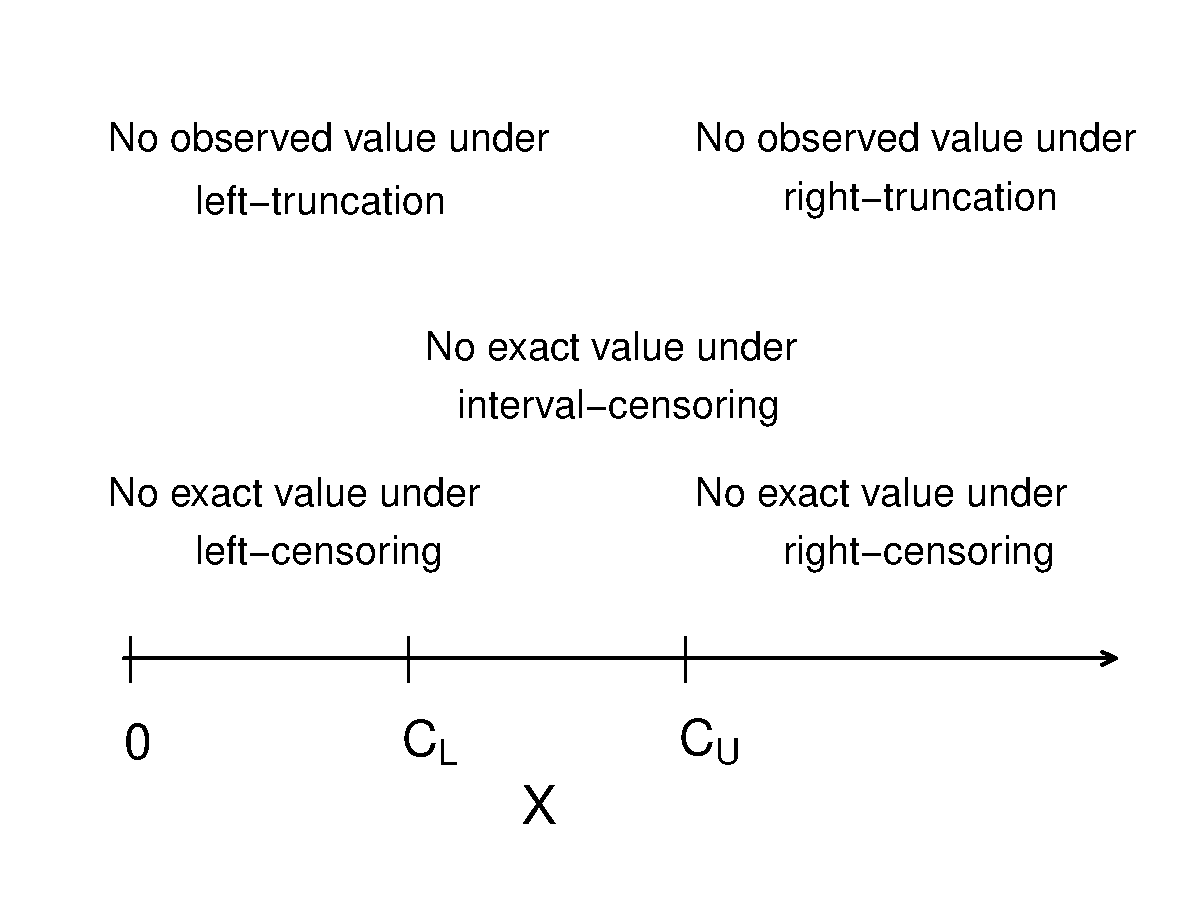
\includegraphics[width=.6\textwidth]{Figures/CensoringTrucation.pdf}
\end{center}
\end{figure}
\end{frame}



\begin{frame}%[shrink=2]
\frametitle{Example: Mortality Study}
\begin{itemize} \scalefont{0.75}
\item Suppose that you are conducting a two-year study of mortality of high-risk subjects, beginning January
1, 2010 and finishing January 1, 2012.
\item For each subject, the beginning of the arrow represents that the the subject was recruited and the arrow end represents the event time. Thus, the
arrow represents exposure time.
\end{itemize}
\vspace{-.1in}
\begin{figure}[htp]
  \begin{center}
    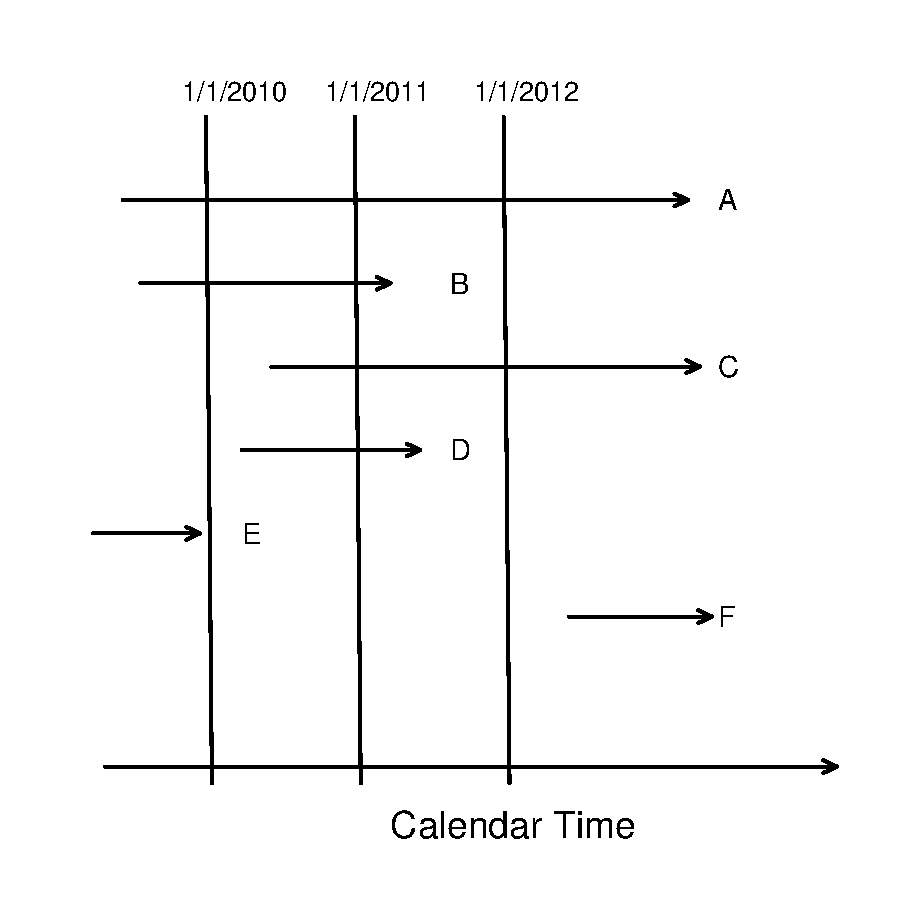
\includegraphics[width=.5\textwidth]{Figures/F14Mortality.pdf}
    %\caption{\label{F14:Mortality}\small Timeline for Several Subjects in a Mortality Study.}
  \end{center}
\end{figure}
\end{frame}


\begin{frame}%[shrink=2]
\frametitle{Example: Mortality Study}
\begin{itemize}\scalefont{0.7}
\item Type A - \textbf{right-censored}. This subject is alive at the beginning and the end of the study. Because the time of death is not known by the end of the study, it is right-censored. Most subjects are Type A.
\item Type B. \textbf{Complete information} is available for a type B subject. The subject is alive at the beginning of the study and the death occurs within the observation period.
\item Type C - \textbf{right-censored} and \textbf{left-truncated}. A type C subject is right-censored, in that death occurs after the observation period. However, the subject entered after the start of the study and is said to have a \emph{delayed entry time}. Because the subject would not have been observed had death occurred before entry, it is left-truncated.
\end{itemize}
\vspace{-.15in}
\begin{figure}[htp]
  \begin{center}
    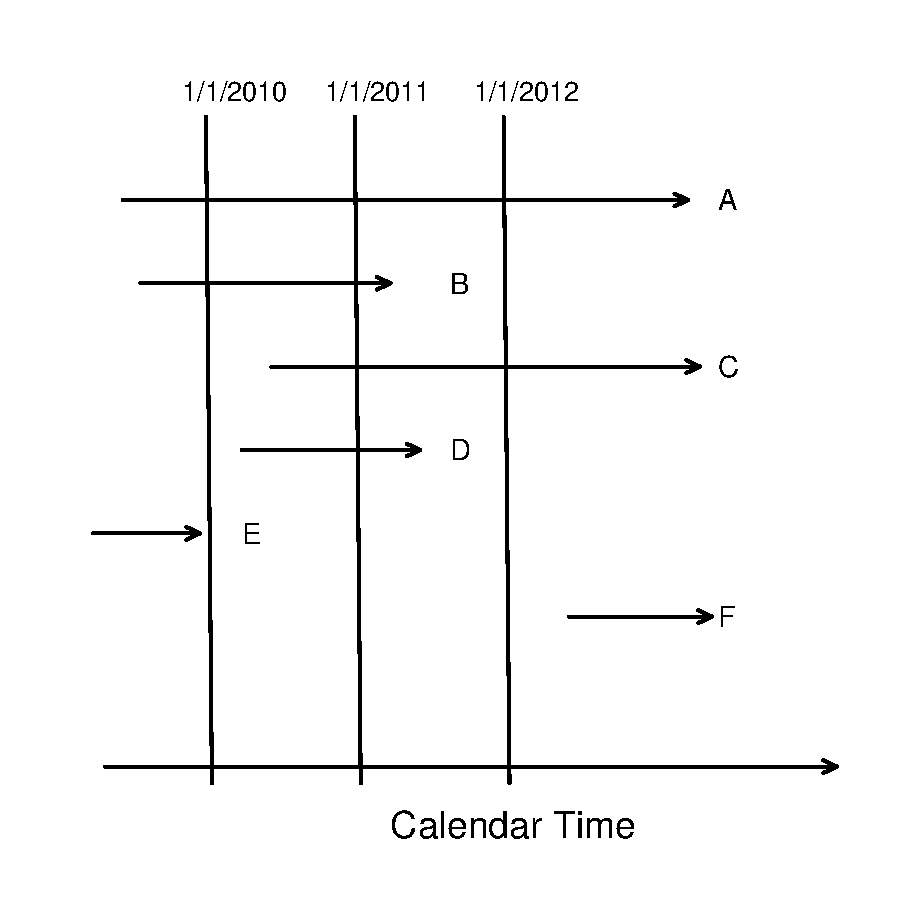
\includegraphics[width=.45\textwidth]{Figures/F14Mortality.pdf}
  \end{center}
\end{figure}
\end{frame}

\begin{frame}%[shrink=2]
\frametitle{Example: Mortality Study}
\begin{itemize}\scalefont{0.7}
\item Type D - \textbf{left-truncated}. A type D subject also has delayed entry. Because death occurs within the observation period, this subject is not right censored.
\item Type E - \textbf{left-truncated}. A type E subject is not included in the study because death occurs prior to the observation period.
\item Type F - \textbf{right-truncated}. Similarly, a type F subject is not included because the entry time occurs after the observation period.
\end{itemize}
\vspace{-.1in}
\begin{figure}[htp]
  \begin{center}
    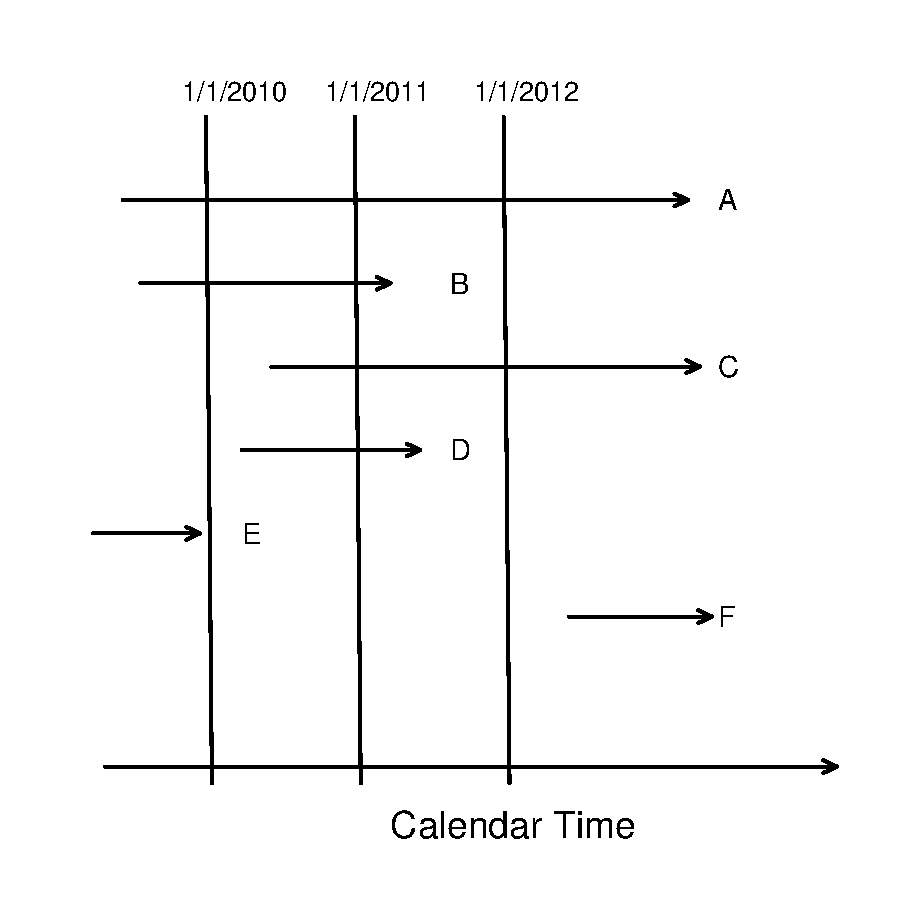
\includegraphics[width=.5\textwidth]{Figures/F14Mortality.pdf}
  \end{center}
\end{figure}
\end{frame}


\subsection{Parametric Estimation Using Censored and Truncated Data}



\begin{frame}[shrink=2]
\frametitle{Maximum Likelihood Estimation Using Censored and Truncated Data}
\begin{itemize}
\item Truncated data are handled in likelihood inference via conditional probabilities \vspace{2mm}

\item Adjust the likelihood contribution by dividing by the probability that the variable was observed \vspace{2mm}

\item Summarizing, we have the following contributions to the likelihood for six types of outcomes \vspace{2mm}

\end{itemize}
\begin{center}
\scalefont{0.9}
\begin{tabular}{lc}
\hline Outcome            & Likelihood~Contribution \\\hline
exact~value        & f($x$) \\
right-censoring    & 1-F($C_U$) \\
left-censoring     & F($C_L$) \\
right-truncation   & f($x$)/F($C_U$) \\
left-truncation    & f($x$)/(1-F($C_L$)) \\
interval-censoring & F($C_U$)-F($C_L$) \\
\hline
\end{tabular}\end{center}
\end{frame}

\begin{frame}[shrink=2]
\frametitle{Maximum Likelihood Estimation Using Censored and
Truncated Data II}
\begin{itemize}
\item For known outcomes and censored data, the likelihood is \vspace{2mm}

\begin{equation*}
\prod_{E} \mathrm{f}(x_i) \prod_{R} \{1-\mathrm{F}(C_{Ui})\}
\prod_{L} \mathrm{F}(C_{Li}) \prod_{I}
(\mathrm{F}(C_{Ui})-\mathrm{F}(C_{Li})),
\end{equation*}
where ``$\prod_{E}$'' is the product over observations with
\textit{E}xact values, and similarly for \textit{R}ight-,
\textit{L}eft- and \textit{I}nterval-censoring \vspace{2mm}

\item For right-censored and left-truncated data, the likelihood is
\begin{equation*}
\prod_{E} \frac{\mathrm{f}(x_i)}{1-\mathrm{F}(C_{Li})} \prod_{R}
\frac{1-\mathrm{F}(C_{Ui})}{1-\mathrm{F}(C_{Li})} ,
\end{equation*} \vspace{2mm}

\item Similarly for other combinations
\end{itemize}
\end{frame}


\begin{frame}%[shrink=2]
\frametitle{Special Case: Exponential Distribution}
\begin{itemize}\scalefont{0.8}
\item Consider data that are right-censored and left-truncated, with random variables $X_i$ that are exponentially distributed with mean $\theta$.
\item With these specifications, recall that $\mathrm{f}(x) = \theta^{-1} \exp(-x/\theta)$ and $\mathrm{F}(x) = 1-\exp(-x/\theta)$.
\item For this special case, the logarithmic likelihood is
\begin{eqnarray*}
 \ln Likelihood  &=& \sum_{E} \left( \ln \mathrm{f}(x_i) - \ln (1-\mathrm{F}(C_{Li})) \right) -\sum_{R}\left( \ln (1-\mathrm{F}(C_{Ui}))- \ln (1-\mathrm{F}(C_{Li}))
 \right) \\
 &=&  \sum_{E} (-\ln \theta -(x_i-C_{Li})/\theta ) -\sum_{R} (C_{Ui}-C_{Li})/\theta .
\end{eqnarray*}
\item To simplify the notation, define $\delta_i = \mathrm{I}(X_i \geq C_{Ui})$ to be a binary variable that indicates right-censoring.
\item Let $X_i^{\ast \ast} = \min(X_i, C_{Ui}) - C_{Li}$ be the amount that the observed variable exceeds the lower truncation limit.
\item With this, the logarithmic likelihood is
\begin{equation*}
 \ln Likelihood =  - \sum_{i=1}^n \left((1-\delta_i) \ln \theta + \frac{x_i^{\ast \ast}}{\theta} \right).
\end{equation*}
\item Taking derivatives with respect to the parameter $\theta$ and setting it equal to zero yields the maximum likelihood estimator
\begin{eqnarray*}
\widehat{\theta}  &=& \frac{1}{n_u} \sum_{i=1}^n  x_i^{\ast \ast},
\end{eqnarray*}
where $n_u = \sum_i (1-\delta_i)$ is the number of uncensored observations.
\end{itemize}
\end{frame}


\section{Bayesian Inference}

\subsection{Bayesian Model}

\begin{frame}%[shrink=.22]
\frametitle{Bayesian Inference}
\begin{itemize}
\item In the \textbf{frequentist interpretation},  one treats the vector of parameters $\boldsymbol \theta$ as fixed yet unknown, whereas the outcomes $X$ are realizations of random variables.
\item With Bayesian statistical models, one views both the model parameters and the data as random variables.
\begin{itemize} \item Use probability tools to reflect this uncertainty about the parameters $\boldsymbol \theta$. \end{itemize}
\item For notation, we will think about $\boldsymbol \theta$ as a random
vector and let $\pi(\boldsymbol \theta)$ denote the distribution of possible
outcomes.
\end{itemize}
\end{frame}


\begin{frame}%[shrink=.22]
\frametitle{Bayesian Inference Strengths}
There are several advantages of the Bayesian approach.
\begin{enumerate}
\item One can describe the entire distribution of parameters conditional on the data. This allows one, for example, to provide probability statements regarding the likelihood of parameters.
\item This approach allows analysts to blend information known from other sources with the data in a coherent manner. This topic is developed in detail in the credibility chapter.
\item The Bayesian approach provides for a unified approach for estimating parameters. Some non-Bayesian methods, such as least squares, required a approach to estimating variance components. In contrast, in Bayesian methods, all parameters can be treated in a similar fashion. Convenient for explaining results to consumers of the data analysis.
\item Bayesian analysis is particularly useful for forecasting future responses.
\end{enumerate}
\end{frame}


\begin{frame}[shrink=.22]
\frametitle{Bayesian Model}
\begin{itemize}
\item \textbf{Prior Distribution.} $\pi(\boldsymbol \theta)$  is called the \textit{prior distribution}.
\begin{itemize}
\item Typically, it is a regular distribution and so integrates to one.
\item We may be very uncertain (or have no clue) about the distribution of $\boldsymbol \theta$; the Bayesian machinery allows this situation
$$ \int \pi(\theta) d\theta = \infty $$
in which case $\pi(\cdot)$ is called an \textbf{improper prior}.
\end{itemize}
\item \textbf{Model Distribution.} The distribution of outcomes given an assumed value of $\boldsymbol \theta$ is known as the \textit{model distribution} and denoted as $f(x | \boldsymbol \theta) = f_{X|\boldsymbol \theta} (x|\boldsymbol \theta )$. This is the (usual frequentist) mass or density function.
\item \textcolor{lightgray}{Joint Distribution}
\item \textcolor{lightgray}{Marginal Outcome Distribution}
\item \textcolor{lightgray}{Posterior Distribution of Parameters}
\end{itemize}
\end{frame}

\begin{frame}%[shrink=2]
\frametitle{Bayesian Model}
\begin{itemize}
\item \textcolor{lightgray}{Prior Distribution}
\item \textcolor{lightgray}{Model Distribution}
\item \textbf{Joint Distribution.} The distribution of outcomes and model parameters is, not surprisingly, known as the \textit{joint distribution} and denoted as $f(x , \boldsymbol \theta) = f(x|\boldsymbol \theta )\pi(\boldsymbol \theta)$.
\item \textbf{Marginal Outcome Distribution.} The distribution of outcomes can be expressed as
$$f(x) =\int f(x | \boldsymbol \theta)\pi(\boldsymbol \theta) d\boldsymbol \theta.$$
This is analogous to a frequentist mixture distribution.
\item \textcolor{lightgray}{Posterior Distribution of Parameters}
\end{itemize}

\end{frame}

\begin{frame}[shrink=.22]
\frametitle{Bayesian Model}
\begin{itemize}
\item \textcolor{lightgray}{Prior Distribution}
\item \textcolor{lightgray}{Model Distribution}
\item \textcolor{lightgray}{Joint Distribution}
\item \textcolor{lightgray}{Marginal Outcome Distribution}
\item \textbf{Posterior Distribution of Parameters.} After outcomes have been observed (hence the terminology ``posterior''), one can use Bayes theorem to write the distribution as
$$ \pi(\boldsymbol \theta | x) =\frac{f(x , \boldsymbol \theta)}{f(x)} =\frac{f(x|\boldsymbol \theta )\pi(\boldsymbol \theta)}{f(x)} $$
The idea is to update your knowledge of the distribution of $\boldsymbol \theta$ ($\pi(\boldsymbol \theta)$) with the data $x$.
\begin{itemize}
\item We can summarize the distribution using a confidence interval type statement.
\item\textbf{Definition}. $[a,b]$ is said to be a $100(1-\alpha)\%$ \textbf{credibility interval} for $\boldsymbol \theta$  if
$$\Pr (a \le \theta \le b | \mathbf{x}) \ge 1- \alpha.$$
\end{itemize}
\end{itemize}
\end{frame}



\begin{frame}[shrink=2]
\frametitle{Two Examples}

\noindent\textbf{Exam C Question 157.} You are given: \\
(i) In a portfolio of risks, each policyholder can have at most one claim per year. \\
(ii) The probability of a claim for a policyholder during a year is $q$. \\
(iii) The prior density is
$$ \pi(q) = q^3/0.07, \ \ \ 0.6 < q < 0.8$$
A randomly selected policyholder has one claim in Year 1 and zero claims in Year 2. \\
For this policyholder, calculate the posterior probability that $0.7 < q < 0.8$.

\bigskip

\noindent\textbf{Exam C Question 43.} You are given: \\
(i) The prior distribution of the parameter $\Theta$ has probability density function:
$$ \pi(\theta) = 1/\theta^2, \ \ \ \ 1 < \theta < \infty$$
(ii) Given $\Theta = \theta$, claim sizes follow a Pareto distribution with parameters $\alpha=2$ and $\theta$.\\
A claim of 3 is observed.\\
Calculate the posterior probability that $\Theta$ exceeds 2.

\end{frame}

\subsection{Bayesian Inference}

\begin{frame}[shrink=2]
\frametitle{Decision Analysis}
\begin{itemize}
\item In classical decision analysis, the loss function $l(\hat{\theta}, \theta)$ determines the penalty paid for using the estimate $\hat{\theta}$ instead of the true $\theta$.
\item The \textbf{Bayes estimate} is that value that minimizes the expected loss $\mathrm{E~}l(\hat{\theta}, \theta)$.
\item Some important special cases include:
\begin{table}[H]\begin{center}\scalefont{0.9}\begin{tabular}{ccc}  \hline
Loss function $l(\hat{\theta}, \theta)$ & Descriptor & Bayes Estimate\\ \hline
$(\hat{\theta}- \theta)^2$ & squared error loss & $\mathrm{E}(\theta|X) $ \\
$|\hat{\theta}- \theta|$ & absolute deviation loss & median of $\pi(\theta|x)$\\
$I(\hat{\theta} =\theta)$ & zero-one loss (for discrete probabilities)& mode of $\pi(\theta|x)$ \\  \hline
\end{tabular}\end{center}\end{table}
\item For new data $y$, the predictive distribution is
$$ f(y|x) = \int f(y|\theta) \pi(\theta|x) d\theta .$$
\item With this, the Bayesian prediction of $y$ is
\begin{eqnarray*}
\mathrm{E}(y|x) &=& \int y f(y|x) dy = \int y \left(\int f(y|\theta) \pi(\theta|x) d\theta \right) dy \\
&=& \int  \mathrm{E}(y|\theta) \pi(\theta|x) d\theta .
\end{eqnarray*}
\end{itemize}
\end{frame}

\begin{frame}[shrink=2]
\frametitle{Posterior Distribution}
How to calculate the posterior distribution?

\begin{itemize}
\item \textbf{By hand} - can do this in special cases
\item \textbf{Simulation} - uses modern computational techniques. \textbf{KPW} (Section 12.4.4) mentions Markov Chain Monte Carlo (MCMC) simulation
\item \textbf{Normal Approximation}. Theorem 12.39 of \textbf{KPW} provides a justification
\item \textbf{Conjugate distributions}. Classical approach. Although this approach is available only for a limited number of distributions, it has the appeal that it provides closed-form expressions for the distributions, allowing for easy interpretations of results. We focus on this approach.
\end{itemize}
To relate the prior and posterior distributions of the parameters, we have
\begin{eqnarray*}
\pi(\boldsymbol \theta | x)&=&\frac{f(x|\boldsymbol \theta )\pi(\boldsymbol \theta)}{f(x)} \\
& \propto & f(x|\boldsymbol \theta ) \pi(\boldsymbol \theta) \\
\text{Posterior} &\text{is proportional to}&\text{likelihood} \times \text{prior}
\end{eqnarray*}
For \textbf{conjugate distributions}, the posterior and the prior come from the same family of distributions.
\end{frame}

\begin{frame}[shrink=2]
\frametitle{Poisson--Gamma Conjugate Family}
\begin{itemize}
\item Assume a Poisson($\lambda$) model distribution so that
$$f(\mathbf{x} | \lambda) = \prod_{i=1}^n \frac{\lambda^{x_i} e^{-\lambda}}{x_i!}$$
\item Assume $\lambda$ follows a gamma($\alpha, \theta$) prior distribution so that
$$\pi(\lambda) = \frac{\left(\lambda/\theta\right)^{\alpha} \exp(-\lambda/\theta)}{\lambda \Gamma(\alpha)}.$$
\item The posterior distribution is proportional to
\begin{eqnarray*}
\pi(\lambda | \mathbf{x}) & \propto & f(\mathbf{x}|\theta ) \pi(\lambda) \\
&=& C \lambda^{\sum_i x_i + \alpha -1} \exp(-\lambda (n+1/\theta))
\end{eqnarray*}
where $C$ is a constant.
\item We recognize this to be a gamma distribution with new parameters $\alpha_{new} = \sum_i x_i + \alpha$ and
$\theta_{new} = 1/(n + 1/\theta)$.
\end{itemize}
\end{frame}


\end{document}
\begin{frame}[shrink=2]
\frametitle{xxx}
\begin{itemize}
\item
\end{itemize}
\end{frame}



\textcolor{blue}{temp}

